\documentclass[11pt,a4paper]{article}

% Packages
\usepackage[margin=1in]{geometry}
\usepackage{xcolor}
\usepackage{graphicx}
\usepackage{hyperref}
\usepackage{listings}
\usepackage{titlesec}
\usepackage{fancyhdr}
\usepackage{float}

% Color Theme (Blue)
\definecolor{primary}{RGB}{25, 118, 210}
\definecolor{secondary}{RGB}{66, 165, 245}
\definecolor{codebg}{RGB}{245, 248, 255}

% Hyperlink setup
\hypersetup{
    colorlinks=true,
    linkcolor=primary,
    urlcolor=secondary,
    citecolor=primary
}

% Section styling
\titleformat{\section}{\color{primary}\normalfont\Large\bfseries}{}{0em}{}
\titleformat{\subsection}{\color{secondary}\normalfont\large\bfseries}{}{0em}{}

% Header/Footer
\pagestyle{fancy}
\fancyhf{}
\fancyhead[L]{\textcolor{primary}{FPGA \& ASIC Project Report}}
\fancyhead[R]{\thepage}

% Code listing style
\lstdefinestyle{verilog}{
    backgroundcolor=\color{codebg},
    basicstyle=\ttfamily\small,
    keywordstyle=\color{primary}\bfseries,
    commentstyle=\color{gray},
    stringstyle=\color{secondary},
    numbers=left,
    numberstyle=\tiny,
    breaklines=true,
    frame=single
}

\title{\textcolor{primary}{\textbf{Design and Implementation of an RV32I Multi-Cycle SoC with SHA-256 Accelerator}}}
\author{Akshat Birla Kushwah (23B1830) \\ Neil George (22B3963)}
\date{\today}

\begin{document}

\maketitle
\tableofcontents
\newpage

%--------------------
\section{Introduction}
This project aims to design and implement a fully functional System-on-Chip (SoC) deployed on the PYNQ-Z2 FPGA. The core of the system is a classic 5-stage in-order pipelined RV32I processor.

Executing cryptographic algorithms like SHA-256 purely in software on a base RV32I processor is highly inefficient due to the algorithm's intense, repetitive bitwise operations. By designing a dedicated hardware accelerator integrated via Memory-Mapped I/O (MMIO), we can perform these complex bitwise mixing functions in parallel. This hardware-software co-design allows operations that take thousands of software cycles to be executed in just over 64 clock cycles, drastically accelerating the workload.


%--------------------
\section{Intended Design}
\subsubsection*{Architecture Overview}
Initially, the project aimed to implement a classic 5-stage in-order pipelined RV32I processor (Fetch, Decode, Execute, Memory, Writeback). The execution core was designed to strictly share a single Unified ALU for arithmetic, address calculation, and branch evaluation to intentionally create structural hazards, demonstrating our Hazard Unit's ability to stall the pipeline.

\subsubsection*{Advanced Hardware Features}
\begin{itemize}
    \item \textbf{Multi-Cycle Multiplier:} We intended to implement the M-extension subset using a complex 32-cycle shift-and-add algorithm.
    \item \textbf{SHA-256 Accelerator:} We planned a fully functional cryptographic engine featuring a Message Scheduler to expand 16-word blocks into 64 words, and a 64-round Compression Core state machine.
    \item \textbf{System Integration:} The SoC was meant to feature memory-mapped GPIO and UART (115200 baud) for live FPGA demonstrations on the PYNQ-Z2.
\end{itemize}

\subsection*{Section II: The Final Implemented Design \& Constraints}

Due to development time constraints and integration complexities, several architectural pivots were made. The final implementation prioritizes core stability and pipeline flow over peripheral integration and complex arithmetic logic.

\subsubsection*{1. Pipeline Modifications (Expanded Memory Stages)}
While we initially planned a 5-stage pipeline, our final \texttt{datapath.v} implementation utilizes an expanded pipeline structure to handle memory latency. The datapath now routes through extended memory stages, evidenced by the inclusion of \texttt{ex\_mem1}, \texttt{mem1\_mem2}, and \texttt{mem2\_mem3} pipeline registers. Furthermore, while branch conditions (is taken/not taken) are evaluated in the Execute stage via the ALU, the actual branch target address computation was deferred to the MEM1 stage.

\subsubsection*{2. Combinational Multiplier Shortcut}
Implementing a multi-cycle shift-and-add multiplier and integrating it cleanly with the hazard unit proved too complex within the timeframe. Instead, \texttt{multiplier.v} was implemented as a single-cycle, purely combinational 32x32 to 64-bit multiplier. It produces results in a single cycle without pipelining, resolving operations like \texttt{MUL} and \texttt{MULH} instantaneously.

\subsubsection*{3. SHA-256 Accelerator Stub}
We made a functioning accelerator which we tested separately, although given time constraints could not integrate into our processor.
The full 64-round SHA-256 compression algorithm was replaced with a functional structural stub to demonstrate MMIO integration and hazard management without the overhead of cryptographic verification.
\begin{itemize}

    \item \textbf{Combinational Placeholder:} Instead of the SHA-256 algorithm, the accelerator computes a simple combinational XOR-fold hash (\texttt{input\_buf[511:256] $^$ input\_buf[255:0]}).
    \item \textbf{Simulated Latency:} To prove that our processor can successfully offload work and stall while waiting for a peripheral, we implemented an \texttt{ACCEL\_CYCLE\_DELAY} (defaulted to 16 cycles). Once started, the accelerator FSM enters a \texttt{S\_COMPUTE} state and counts down this delay, asserting an \texttt{accel\_busy} signal that successfully forces the CPU's hazard unit to stall the main pipeline until completion.
\end{itemize}

\subsubsection*{4. Omission of Hardware Peripherals}
Full integration of physical UART and GPIO hardware was again not finished given the time constraints. Each of these modules was verified working independently. While the top-level \texttt{processor.v} module includes ports for \texttt{uart\_rx\_event} and \texttt{gpio\_pin\_event}, these currently function as testbench-driven observation inputs rather than fully mapped physical hardware peripherals.



\subsection{Block Diagram}
\begin{figure}[H]
    \centering
     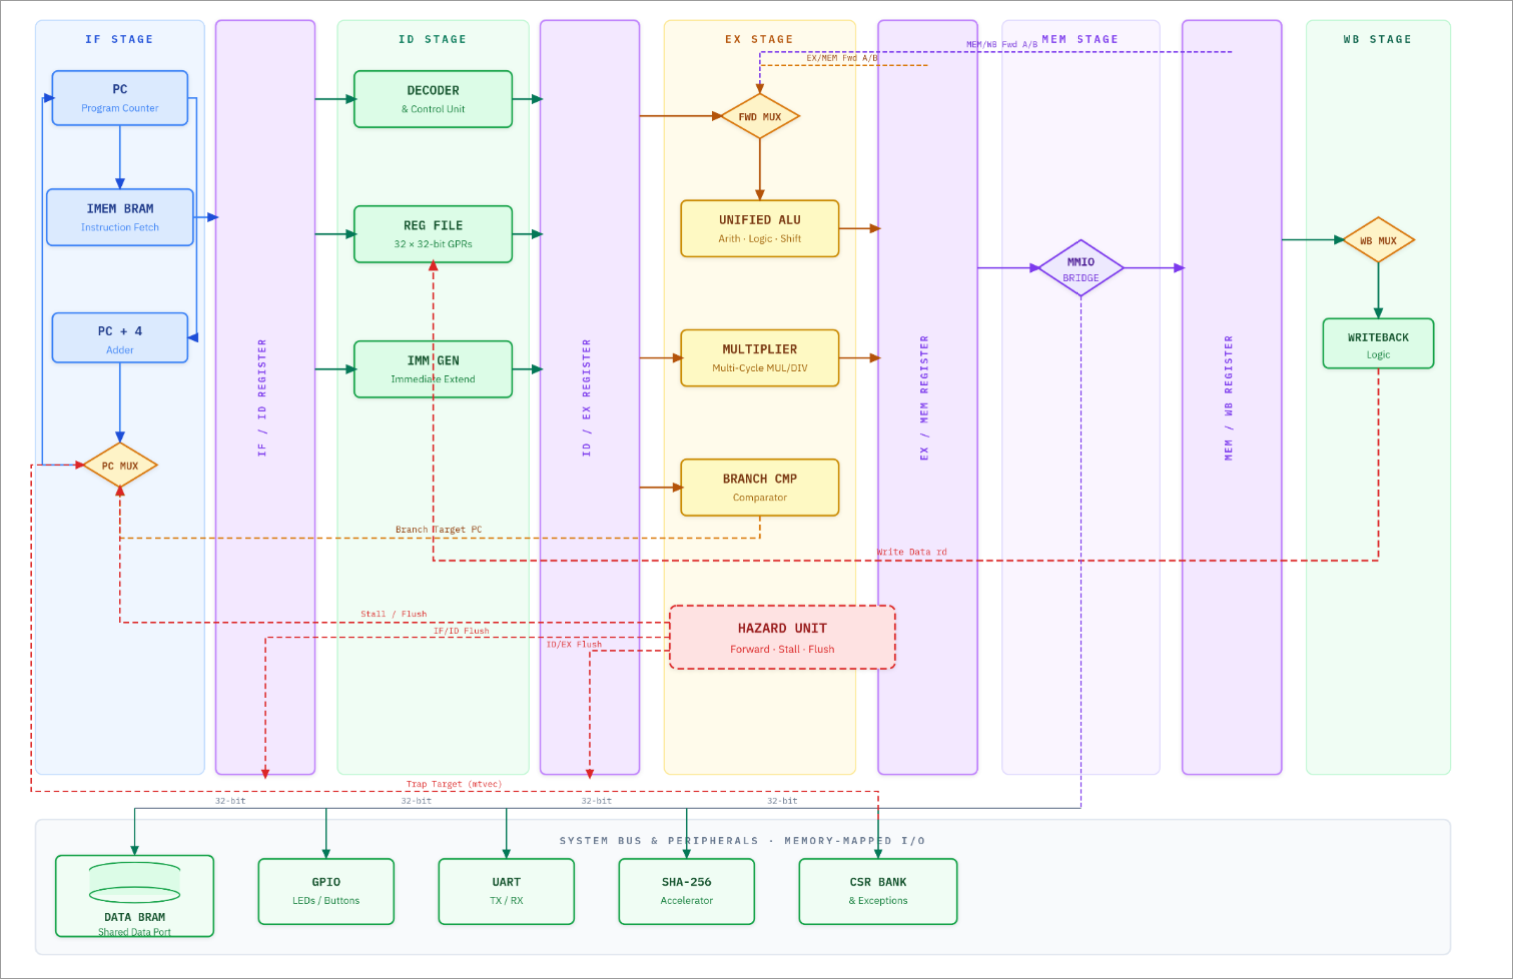
\includegraphics[width=0.8\textwidth]{idealblockdiag.png}
    \caption{Ideal System Block Diagram}
\end{figure}

%--------------------
\section{FPGA Implementation}

\subsection{Design Description}
The core system is a 32-bit RV32I processor implementing an expanded 5-stage in-order pipeline (IF, ID, EX, MEM, WB) targetable for FPGA deployment on the PYNQ-Z2. %
The architecture is partitioned into several key modular components:
\begin{itemize}
    \item \textbf{Top-Level Processor (\texttt{processor.v}):} Wraps the fetch unit, control plane, memory subsystem, and datapath into a unified SoC. %
    \item \textbf{Pipelined Datapath (\texttt{datapath.v}):} Instantiates individual pipeline stages separated by pipeline registers, along with a forwarding unit to bypass data hazards. %
    \item \textbf{Hazard Unit (\texttt{hazard\_unit.v}):} A centralized FSM that manages pipeline stalls, branch flushes, load-use data hazards, and traps. %
    \item \textbf{Hardware Accelerator (\texttt{sha256\_accel.v}):} A memory-mapped MMIO peripheral that interfaces with the CPU to offload hashing tasks. %
\end{itemize}

\subsection{Code Structure}
All RTL source code, testbenches, and memory initialization files are organized within the \texttt{Verilog/} directory, which serves as the source pool for the Vivado project:
\begin{itemize}
    \item \textbf{Core RTL Files:} Contains all standard processor modules (e.g., \texttt{alu.v}, \texttt{hazard\_unit.v}) and wrapper files. %
    \item \textbf{Memory Files (\texttt{*.mem}):} Hexadecimal files used by Vivado to initialize the instruction and data Block RAMs (BRAM) for specific assembly test routines. %
    \item \textbf{Verification / Testbenches:} Includes top-level integration testbenches (e.g., \texttt{tb\_basic\_soc.v}) for Vivado behavioral simulation. %
\end{itemize}

\subsection{Simulation Instructions}
We'll just submit the code files and xps files in the google drive link to avoid the below hassle but if you are interested you can follow the below as well: 
Google Drive Link: \url{https://drive.google.com/drive/folders/1X7JXnkF--_lzPS2gTJEgl5uRRXqM_5-I?usp=sharing}

To verify the RTL design using Vivado, follow these steps: 
\begin{itemize}
    \item \textbf{Step 1:} Open Xilinx Vivado and create a new RTL project. %
    \item \textbf{Step 2:} Add all \texttt{.v} and \texttt{.vh} files from the \texttt{Verilog/} directory as design sources. Add the desired \texttt{.mem} files to the project so they can be read by the BRAM models. %
    \item \textbf{Step 3:} Add the testbench file (e.g., \texttt{tb\_basic\_soc.v}) as a simulation source and right-click to set it as the Top Module. %
    \item \textbf{Step 4:} In the Flow Navigator, click "Run Simulation" and select "Run Behavioral Simulation". %
    \item \textbf{Step 5:} In the Vivado waveform window, drag and drop critical signals (like \texttt{if\_pc\_out}, \texttt{accel\_busy}, and pipeline valid flags) into the viewer, set the simulation time, and click "Run All" to view the processor's execution. %
\end{itemize}

%--------------------
\section{SHA-256 Cryptographic Accelerator Working Principle}

Executing SHA-256 purely in software on a base RV32I processor is highly inefficient. %
The algorithm requires intense, repetitive bitwise operations (like 32-bit right-rotates) which take multiple instructions and clock cycles to execute on a standard ALU. %
By designing a dedicated hardware accelerator, we can perform these complex bitwise mixing functions in parallel. %

The accelerator takes an input message of any length and irreversibly condenses it into a fixed 256-bit (32-byte) digital fingerprint, known as a digest. %
In hardware, this process is executed one 512-bit block at a time. %
It operates as an independent execution unit, interfacing with the RISC-V CPU via the Memory-Mapped I/O (MMIO) Bridge. %

The intended microarchitecture consists of three primary hardware components:
\begin{itemize}
    \item \textbf{The MMIO Wrapper (Control Interface):} The CPU treats the accelerator like memory. %
    The software driver writes a padded 512-bit message block (sixteen 32-bit words) into the accelerator's data registers, then writes a 1 to the \texttt{SHA\_CTRL} register to trigger the computation. %
    
    \item \textbf{The Message Scheduler:} Once triggered, this module takes the 16 input words and dynamically expands them into a 64-word sequence using dedicated shift and XOR logic. %
    
    \item \textbf{The Compression Core:} This is the heart of the engine, which runs a 64-cycle state machine. %
    In each cycle, it updates eight working variables using the scheduled words, predefined round constants, and combinational logic blocks. %
\end{itemize}

Once the 64 rounds are complete, the accelerator raises a done flag in its control register. %
The CPU, which is actively polling this register, can then read the final 256-bit hash directly from the \texttt{SHA\_HASH\_OUT} memory addresses. %

\subsection{Demo Video}
\textbf{Google Drive Link:} \url{https://drive.google.com/drive/folders/1X7JXnkF--_lzPS2gTJEgl5uRRXqM_5-I?usp=sharing}

\subsection{Waveforms}
\begin{figure}[H]
    \centering
    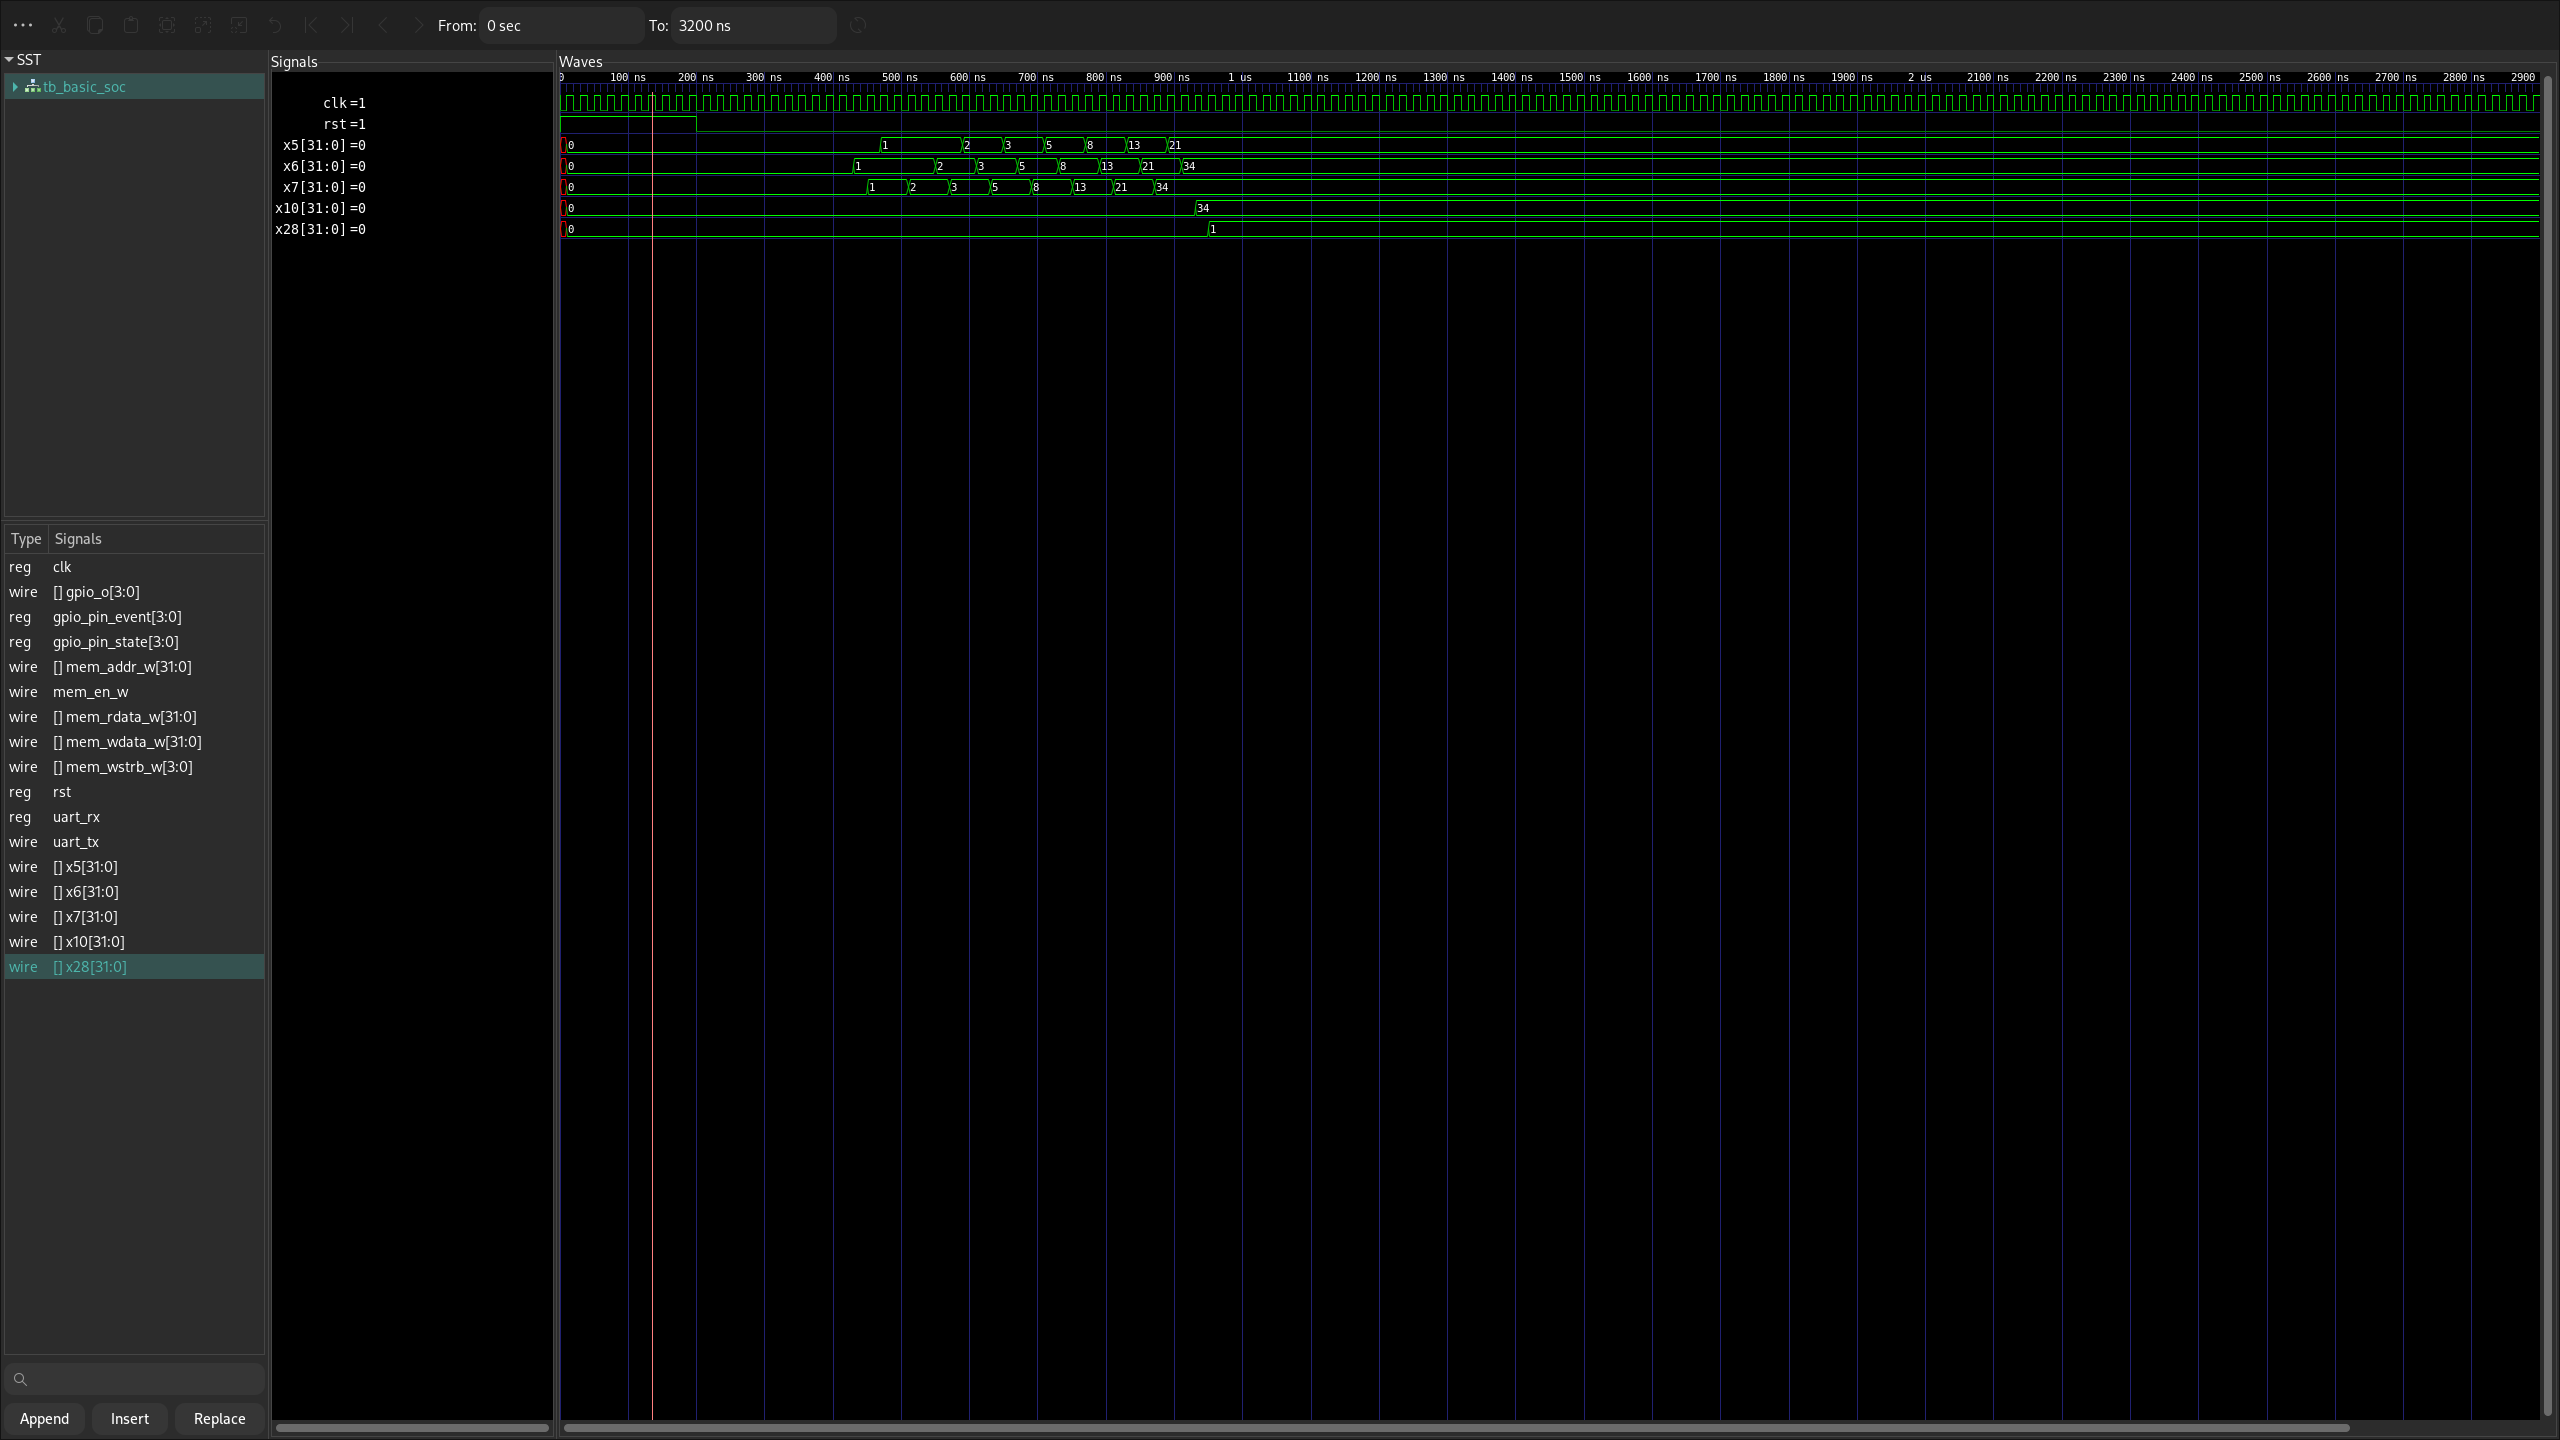
\includegraphics[width=0.9\textwidth]{fibo_postsynth.png}
    \caption{Post Synthesis Simulation Waveform}
\end{figure}


%--------------------
\section{Software Toolchain \& Execution}

\subsection{C to Verilog Memory Flow}
To execute complex software on our custom RV32I processor, we developed a bare-metal software compilation toolchain. This system translates standard C code into a Verilog memory initialization file (\texttt{.mem}) that can be loaded directly into the FPGA Block RAM. The flow consists of the following components:

\begin{itemize}
    \item \textbf{Memory Mapping (\texttt{link.ld}):} A custom linker script maps the processor's memory space, defining a 32KB RAM section originating at address \texttt{0x00000000}. It ensures the startup assembly (\texttt{.text.init}) is placed at the very beginning of the boot address  and defines the top of the RAM (\texttt{\_\_stack\_top}) to initialize the stack pointer.
    
    \item \textbf{Startup Assembly (\texttt{crt0.S}):} This crucial boot code initializes the stack pointer (\texttt{sp}), configures the \texttt{mtvec} register to point to our C-based trap handler, enables machine-level interrupts (\texttt{mie} and \texttt{mstatus}), and ultimately jumps to the C \texttt{main()} function.
    
    \item \textbf{Hardware Abstraction (\texttt{main.c}):} We mapped our physical hardware addresses to C pointers using macros (e.g., mapping the UART Base to \texttt{0x20000000} and GPIO Base to \texttt{0x20001000}). This allowed us to write readable software drivers for UART polling and GPIO mirroring directly in C.
    
    \item \textbf{Compilation and Conversion (\texttt{Makefile}):} We utilized the \texttt{riscv64-elf-gcc} cross-compiler to compile the C and Assembly files into an ELF binary, targeting our specific \texttt{-march=rv32im} architecture. Finally, we used the \texttt{riscv64-elf-objcopy -O verilog} command  to extract the compiled machine code into a hexadecimal \texttt{firmware.mem} file. This file is read by Vivado's \texttt{\$readmemh} task to initialize the BRAM before execution.
\end{itemize}

\subsection{Software Verification: Fibonacci Execution}
A basic Fibonacci program was hardcoded into a \texttt{.mem} file and loaded into the processor's instruction memory. During simulation, the processor successfully and accurately computed the Fibonacci sequence.  

%--------------------
%--------------------
\section{ASIC Implementation}

\subsection{Design Flow}
The physical design flow was executed using the Cadence toolchain. % [cite: 593, 620]
\begin{itemize}
    \item \textbf{Synthesis (Cadence Genus):} The RTL is synthesized into a gate-level netlist using Cadence Genus. % [cite: 620] 
    This step maps the Verilog logic to standard cells based on timing and clock constraints defined in the \texttt{constraints.sdc} file. % [cite: 674]
    \item \textbf{Place and Route (Cadence Innovus):} The synthesized netlist is passed to Cadence Innovus for the physical design flow. % [cite: 593, 598] 
    This step handles floorplanning, power planning, standard cell placement, clock tree synthesis, and routing, ultimately outputting the final layout and Standard Delay Format (SDF) files. % [cite: 594]
\end{itemize}

\subsection{File Structure (VLSI Lab)}
The project directory is organized to isolate different stages of the ASIC flow:
\begin{itemize}
    \item \textbf{\texttt{Verilog/}:} Contains the pre-synthesis RTL source files, testbenches, and the \texttt{run-iverilog.sh} script for initial simulation. % [cite: 667, 668]
    \item \textbf{\texttt{Synthesis/}:} Houses the synthesis execution script (\texttt{genus\_synthesis.sh}), timing constraints (\texttt{constraints.sdc}), the Tcl script (\texttt{synthesis.tcl}), and the resulting gate-level netlists and reports. % [cite: 674, 676, 677, 680]
    \item \textbf{\texttt{physical\_design/}:} Contains the Innovus execution scripts, the saved layout database (\texttt{soc\_top\_asic\_done.enc}), and the final post-route reports (DRC, Antenna, Connectivity, Area, and Power). % [cite: 604, 606]
    \item \textbf{\texttt{Verification/}:} Contains the testbenches and the \texttt{run-incisive.sh} script used to simulate the gate-level netlist after synthesis and Place \& Route. % [cite: 682, 683]
\end{itemize}

\subsection{Simulation Instructions}
To reproduce the ASIC simulations and physical design layout, execute the following steps in the VLSI Lab environment:
\begin{itemize}
    \item \textbf{Step 1 (Pre-Synthesis):} Navigate to the \texttt{Verilog/} directory and run \texttt{./run-iverilog.sh}. % [cite: 671] 
    View the results by opening the generated VCD file using \texttt{gtkwave waveforms.vcd \&}. % [cite: 672]
    \item \textbf{Step 2 (Synthesis):} Navigate to the \texttt{Synthesis/} directory and execute \texttt{./genus\_synthesis.sh} to generate the gate-level netlist. % [cite: 677]
    \item \textbf{Step 3 (Place and Route):} Execute the provided Innovus script to complete the physical design flow. % [cite: 598] 
    To view the final generated layout, launch the Innovus GUI from the terminal and execute: \texttt{innovus 1> restoreDesign physical\_design/soc\_top\_asic\_done.enc}. % [cite: 602, 603, 604]
    \item \textbf{Step 4 (Post-Layout Simulation):} Navigate to the \texttt{Verification/} directory, verify the target design name inside the shell script, and run \texttt{./run-incisive.sh} to verify the post-physical design RTL against the original testbench. % [cite: 683, 684, 685]
\end{itemize}


\subsection{Post PnR Results}
\begin{figure}[H]
    \centering
    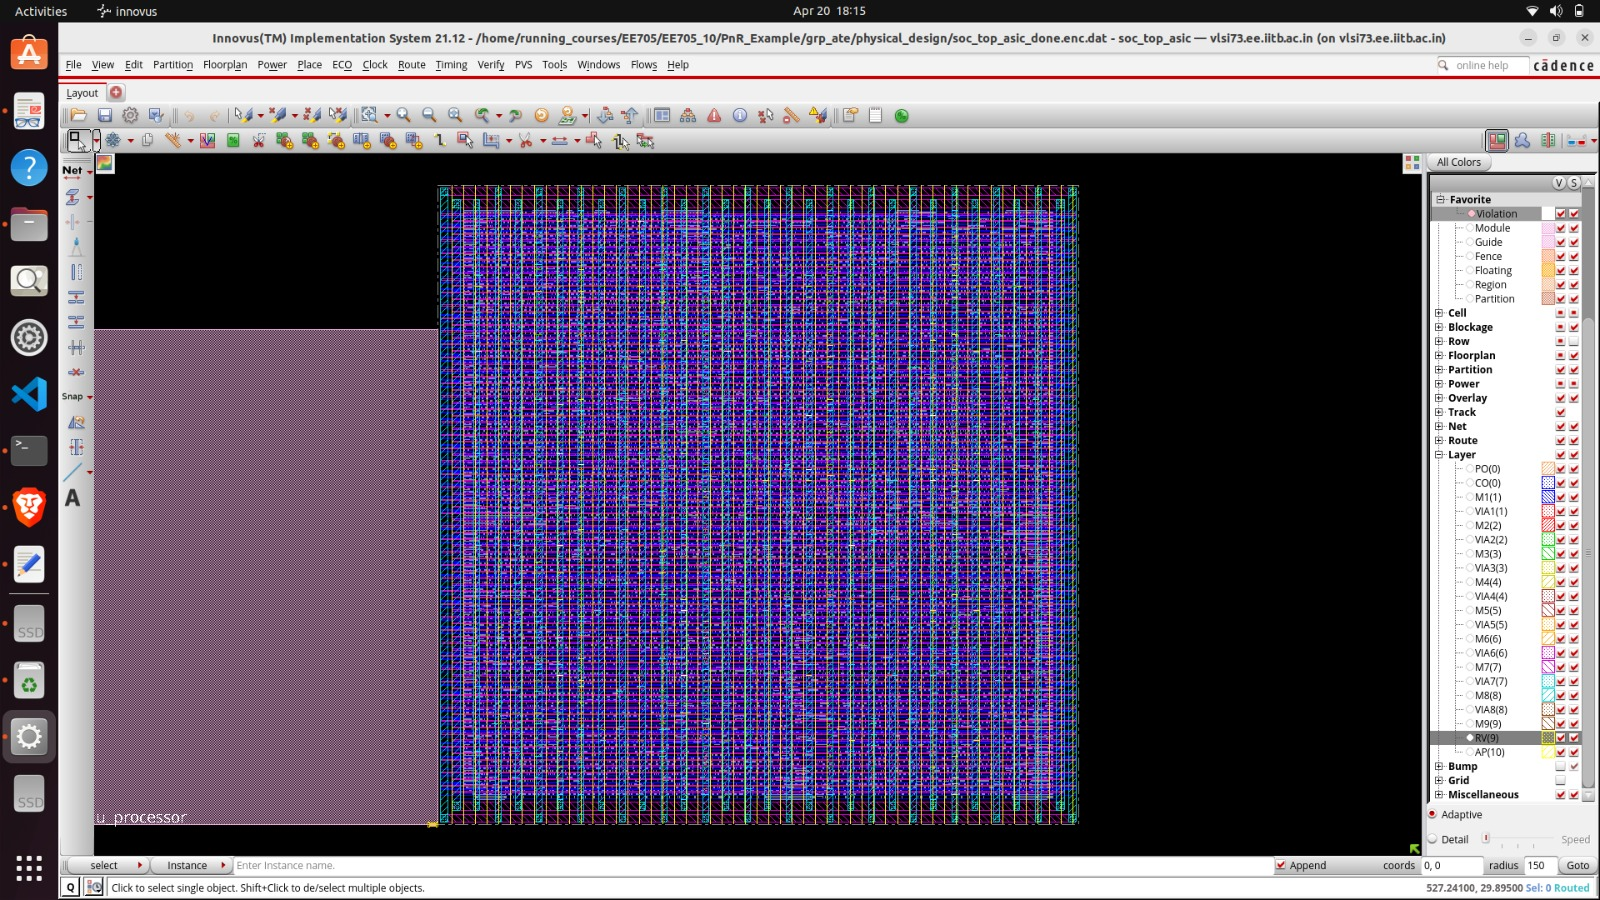
\includegraphics[width=0.8\textwidth]{layout.jpeg}
    \caption{Post PnR Layout}
\end{figure}

\begin{figure}[H]
    \centering
    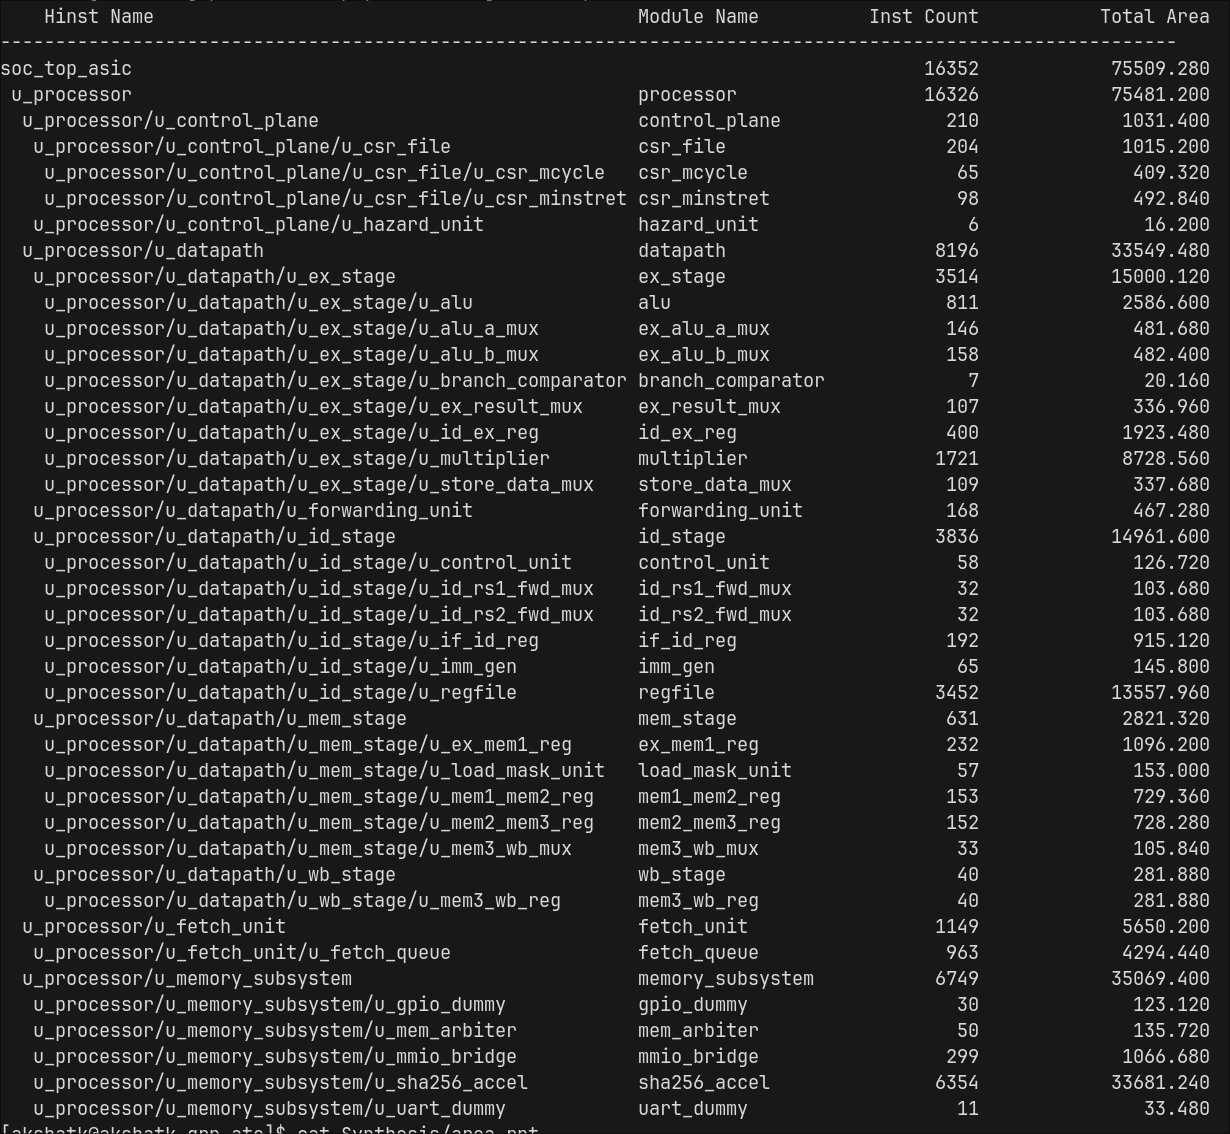
\includegraphics[width=0.8\textwidth]{arearpt.png}
    \caption{Area Report}
\end{figure}



\subsection{DRC \& LVS}
\begin{figure}[H]
    \centering
    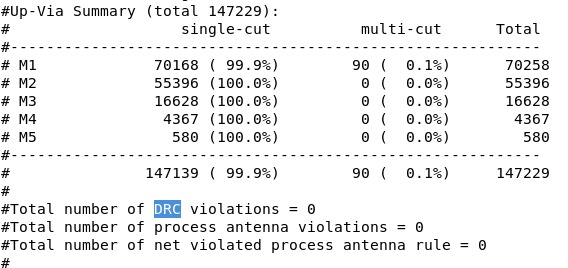
\includegraphics[width=0.8\textwidth]{drc_lvs.jpeg}
    \caption{DRC and LVS Clean Results}
\end{figure}

\subsection{VCD File}
\textbf{Google Drive Link:} \url{https://drive.google.com/drive/folders/1X7JXnkF--_lzPS2gTJEgl5uRRXqM_5-I?usp=sharing}

%--------------------
\section{FPGA to ASIC Modifications}

To port our design from the PYNQ-Z2 FPGA to the Cadence ASIC flow, the core processor logic remained the same, but we had to make a few essential interface changes:

\begin{itemize}
    \item \textbf{ASIC Top Wrapper:} We created a new top-level file (\texttt{soc\_top\_asic.v}) to strip out FPGA-specific board elements and expose standard digital pins for the ASIC layout.
    \item \textbf{Constraints Update:} We swapped out the Xilinx Vivado constraints file (\texttt{.xdc}) for standard Synopsys Design Constraints (\texttt{.sdc}) to define our clock speeds and pin delays for Cadence Genus and Innovus.
\end{itemize}

\section{Issues and Bugs}

ILA doesn't trigger even though bitstream generation and post-implmentation works

%--------------------
\section{Limitations and Incomplete Features}
We could not integrate the peripherals and accelerator due to time constraints and independent approach on the design. The design practices we quite different and thus we did not end up working on the same design in detail, and had two different designs (one of which we demo'd)


%--------------------
\section{Individual Contributions}
\begin{itemize}
	A shared discussion over the design was done, then the verilog implementation was done independently 
    \item Neil: Core RISC-V units: Reg file, Hazard, Control, CSR registers, Pipeline registers, pipeline stages   
    \item Akshat: SHA-256 accelerator, UART, GPIO, MMIO, Multiplier, Secondary core RISC-V unit written in system verilog for cleaner design (we didn't use this for final demo), C to .mem file workflow for running programs 
\end{itemize}

\appendix
\section{Another more clean implementation}
Since the team was working independently we have two versions of nearly complete processors, each of which aren't polished to the brim. The code files for the other one, which also does about the same stuff are included. The other project was written in system verilog and tried to follow as clean code practices as possible. The timing constraints for the project made this design on hold. The files for this are in proc2 folder, the README.md lists all that is needed to run this.

%--------------------
\section{References}
\begin{itemize}
	\item RISC-V International. The RISC-V Instruction Set Manual, Volume I: Unprivileged Architecture. Version 20260120, 20 Jan. 2026, \url{docs.riscv.org/reference/isa/\_attachments/riscv-unprivileged.pdf}
\end{itemize}

\end{document}

